\chapter{Raytracing}
\section{Grundidee}
Raytracing erzeugt fotorealistische Bilder, indem es Spiegelung und Transparenz berechnet. Grundsätzlich generiert man für jeden Pixel eine Linie in das Bild hinein und schaut dann, welches Objekt diese Linie zuerst schneidet. Wenn das erste Objekt gefunden wurde, dann berechne die Farbe. Simpel as that.
\begin{figure}[!ht]
	\centering
	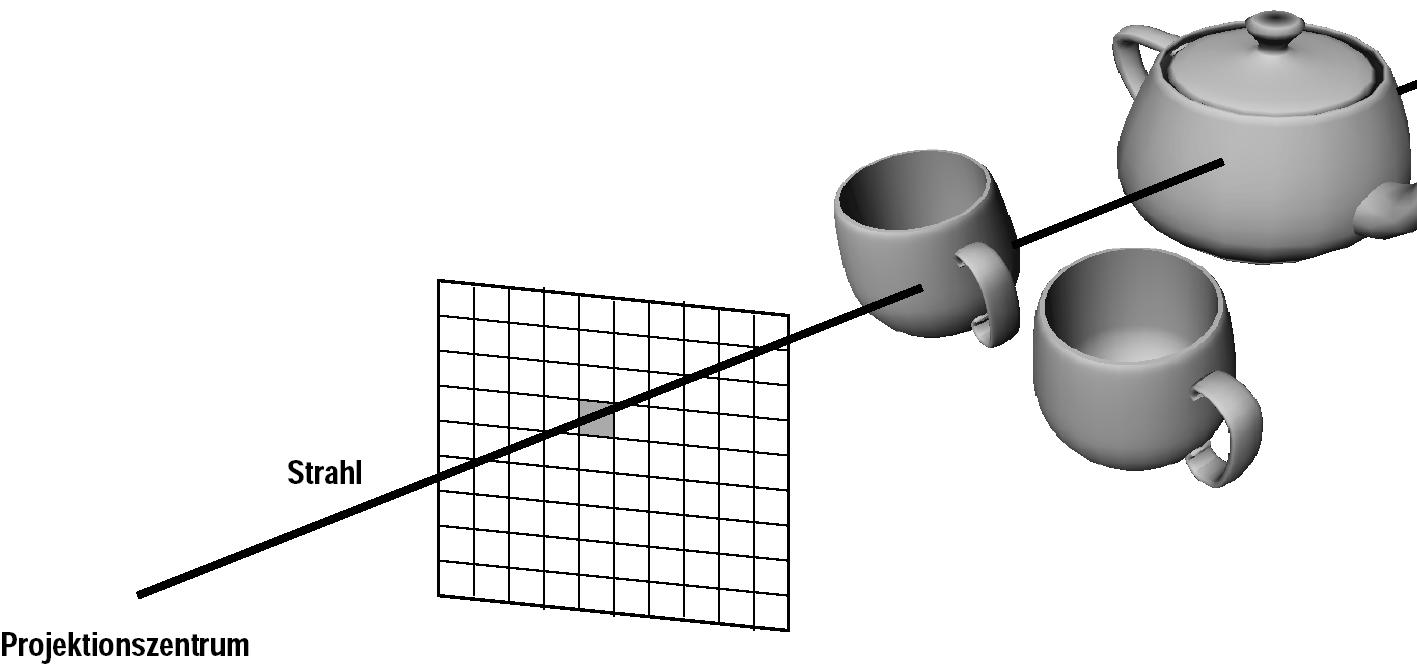
\includegraphics[width=0.4\linewidth]{fig/raytracing}
	\caption{Raytracing Grundidee}
	\label{fig:raytracing}
\end{figure}

\section{Rekursives Raytracing}
Mit dem ersten Strahl auf das Objekt ist noch nicht viel Realität in den PC geholt worden. Erst mit dem rekursiven Raytracing kommt das (Siehe Abbildung \label{fig:raytracing_rekursiv}).
\begin{figure}[!ht]
	\centering
	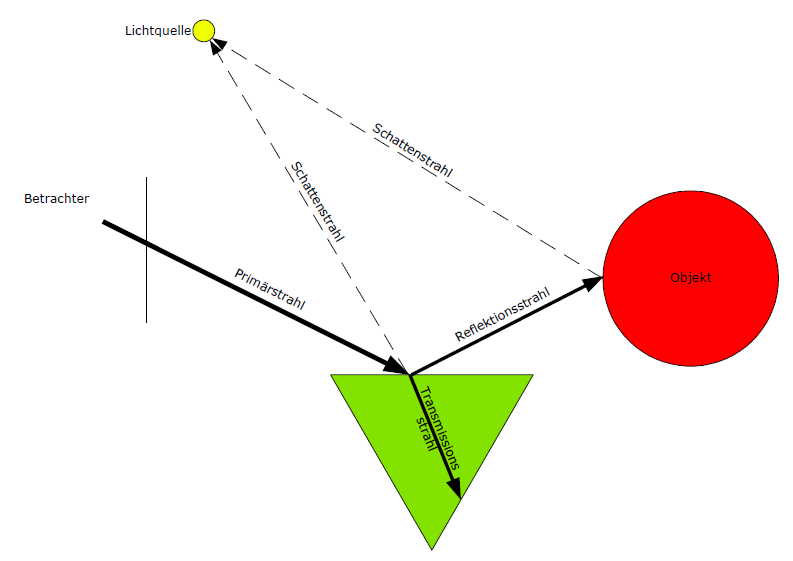
\includegraphics[width=0.8\linewidth]{fig/raytracing_rekursiv}
	\caption{Rekursives Raytracing}
	\label{fig:raytracing_rekursiv}
\end{figure}\\
Wir haben also den ersten Strahl vom Betrachter aus - unseren \textit{Primärstrahl}. Dieser geht vom Betrachter direkt auf den betrachteten Pixel. Von dort aus machen wir weitere Strahlen - einmal ein Reflexionsstrahl, der ähnlich wie der Primärstrahl einfach das nächste Objekt sucht und schaut, was dort für eine Farbe ist und diese dann dem ersten Punkt hinzufügt. Dann gibt es noch die Schattenstrahlen, die von der Lichtquelle aus berechnen, wie sehr diese jetzt den Punkt beleuchten. Dann gibt es no den Transmissionsstrahl, der durch das Objekt hindurch geht, und die Farbe holt, die am anderen Ende des Objekts ist. Wir haben also:
\begin{enumerate}
	\item \textbf{Primärstrahl} - Der erste Strahl vom Betrachter zum Objekt
	\item \textbf{Schattenstrahl} - Der Strahl vom betracheten Punkt zur Lichtquelle
	\item \textbf{Reflektionsstrahl} - Der Strahl der Reflektion
	\item \textbf{Transmissionsstrahl} - Der Strahl der durch das Objekt hindurch geht
\end{enumerate}
Jetzt kommt es natürlich nur noch darauf an, wie tief man diese Strahlen verfolgt. Irgendwann sind sie nur noch so schwach, dass sie fast keinen Einfluss mehr darauf haben, wie das Bild aussieht, deswegen hört man auch irgendwann auf - und auch natürlich wegen der Rechenzeit ist es wichtig, diese \textit{Strahlentiefe} zu begrenzen.

\subsection{Aliasing}
Weil man nicht so schöne Bilder erhält mit dem Raytracing an sich, verwendet man noch ein adaptives Supersampling. Man macht also bis zu 16 Rays pro Pixel und fügt diese dann zu einem Pixel wieder zusammen.